%% Produit par outils/generer.py — ne pas modifier à la main.

\subsection*{The A Family}
\noindent\textbf{Key signature:} three sharps: F$\sharp$, C$\sharp$, G$\sharp$.\smallskip

\begin{center}
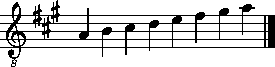
\includegraphics[height=1.15cm]{scale-A.cropped}\\[2pt]
{\small\color{mygray}\textbf{1} A\quad \textbf{2} B\quad \textbf{3} C$\sharp$\quad \textbf{4} D\quad \textbf{5} E\quad \textbf{6} F$\sharp$\quad \textbf{7} G$\sharp$\quad \textbf{8} A}
\end{center}

\begin{longtable}{@{}l l l c >{\raggedright\arraybackslash}p{4.4cm}@{}}
\toprule
\textbf{Symbol} & \textbf{Full name} & \textbf{Formula} & \textbf{Staff} & \textbf{Colour / use} \\
\midrule\endhead
\rowcolor{rowA}
\textbf{A} & A major & 1 -- 3 -- 5 & 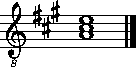
\includegraphics[height=1.15cm]{th-Amaj.cropped} & Bright, stable. \\
\rowcolor{rowB}
\textbf{Am} & A minor & 1 -- $\flat$3 -- 5 & 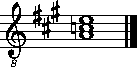
\includegraphics[height=1.15cm]{th-Am.cropped} & Dark. Lower the 3rd: C$\sharp$ $\to$ C. \\
\rowcolor{rowA}
\textbf{A5} & A power chord & 1 -- 5 & 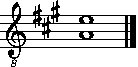
\includegraphics[height=1.15cm]{th-A5.cropped} & Raw, neutral. No 3rd. \\
\rowcolor{rowB}
\textbf{Asus2} & A sus. 2nd & 1 -- 2 -- 5 & 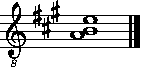
\includegraphics[height=1.15cm]{th-Asus2.cropped} & Open. Replace 3rd with 2nd (B). \\
\rowcolor{rowA}
\textbf{Asus4} & A sus. 4th & 1 -- 4 -- 5 & 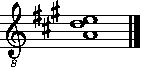
\includegraphics[height=1.15cm]{th-Asus4.cropped} & Tense. Replace 3rd with 4th (D). \\
\rowcolor{rowB}
\textbf{A6} & A major sixth & 1 -- 3 -- 5 -- 6 & 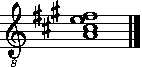
\includegraphics[height=1.15cm]{th-A6.cropped} & Sweet, vintage. Add 6th (F$\sharp$). \\
\rowcolor{rowA}
\textbf{Aadd9} & A add nine & 1 -- 3 -- 5 -- 9 & 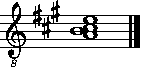
\includegraphics[height=1.15cm]{th-Aadd9.cropped} & Colourful. Add 2nd/9th (B), no 7th. \\
\rowcolor{rowB}
\textbf{A7} & A dominant 7th & 1 -- 3 -- 5 -- $\flat$7 & 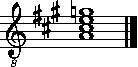
\includegraphics[height=1.15cm]{th-A7.cropped} & Bluesy. Lower 7th: G$\sharp$ $\to$ G. \\
\rowcolor{rowA}
\textbf{Amaj7} & A major 7th & 1 -- 3 -- 5 -- 7 & 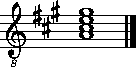
\includegraphics[height=1.15cm]{th-Amaj7.cropped} & Dreamy, jazzy. Keep natural 7th (G$\sharp$). \\
\rowcolor{rowB}
\textbf{Am7} & A minor 7th & 1 -- $\flat$3 -- 5 -- $\flat$7 & 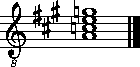
\includegraphics[height=1.15cm]{th-Am7.cropped} & Mellow, soulful. Lower 3rd and 7th. \\
\rowcolor{rowA}
\textbf{Aaug} & A augmented & 1 -- 3 -- $\sharp$5 & 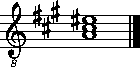
\includegraphics[height=1.15cm]{th-Aaug.cropped} & Eerie. Raise the 5th by 1 semitone. \\
\rowcolor{rowB}
\textbf{Adim} & A diminished & 1 -- $\flat$3 -- $\flat$5 & 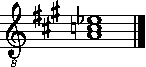
\includegraphics[height=1.15cm]{th-Adim.cropped} & Very tense. Lower 3rd and 5th. \\
\rowcolor{rowA}
\textbf{Adim7} & A dim. 7th & 1 -- $\flat$3 -- $\flat$5 -- $\flat\flat$7 & 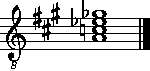
\includegraphics[height=1.15cm]{th-Adim7.cropped} & Max. tense. All minor 3rds. \\
\rowcolor{rowB}
\textbf{Am7$\flat$5} & A half-dim. & 1 -- $\flat$3 -- $\flat$5 -- $\flat$7 & 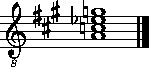
\includegraphics[height=1.15cm]{th-Am7b5.cropped} & Tense, jazzy (also: A\o). \\
\bottomrule
\end{longtable}

\subsection*{The B Family}
\noindent\textbf{Key signature:} five sharps: F$\sharp$, C$\sharp$, G$\sharp$, D$\sharp$, A$\sharp$.\smallskip

\begin{center}
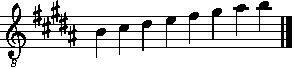
\includegraphics[height=1.15cm]{scale-B.cropped}\\[2pt]
{\small\color{mygray}\textbf{1} B\quad \textbf{2} C$\sharp$\quad \textbf{3} D$\sharp$\quad \textbf{4} E\quad \textbf{5} F$\sharp$\quad \textbf{6} G$\sharp$\quad \textbf{7} A$\sharp$\quad \textbf{8} B}
\end{center}

\begin{longtable}{@{}l l l c >{\raggedright\arraybackslash}p{4.4cm}@{}}
\toprule
\textbf{Symbol} & \textbf{Full name} & \textbf{Formula} & \textbf{Staff} & \textbf{Colour / use} \\
\midrule\endhead
\rowcolor{rowA}
\textbf{B} & B major & 1 -- 3 -- 5 & 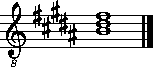
\includegraphics[height=1.15cm]{th-Bmaj.cropped} & Bright, stable. \\
\rowcolor{rowB}
\textbf{Bm} & B minor & 1 -- $\flat$3 -- 5 & 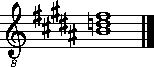
\includegraphics[height=1.15cm]{th-Bm.cropped} & Dark. Lower the 3rd: D$\sharp$ $\to$ D. \\
\rowcolor{rowA}
\textbf{B5} & B power chord & 1 -- 5 & 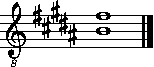
\includegraphics[height=1.15cm]{th-B5.cropped} & Raw, neutral. No 3rd. \\
\rowcolor{rowB}
\textbf{Bsus2} & B sus. 2nd & 1 -- 2 -- 5 & 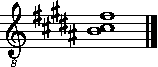
\includegraphics[height=1.15cm]{th-Bsus2.cropped} & Open. Replace 3rd with 2nd (C$\sharp$). \\
\rowcolor{rowA}
\textbf{Bsus4} & B sus. 4th & 1 -- 4 -- 5 & 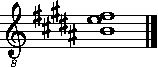
\includegraphics[height=1.15cm]{th-Bsus4.cropped} & Tense. Replace 3rd with 4th (E). \\
\rowcolor{rowB}
\textbf{B6} & B major sixth & 1 -- 3 -- 5 -- 6 & 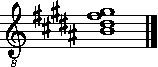
\includegraphics[height=1.15cm]{th-B6.cropped} & Sweet, vintage. Add 6th (G$\sharp$). \\
\rowcolor{rowA}
\textbf{Badd9} & B add nine & 1 -- 3 -- 5 -- 9 & 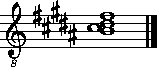
\includegraphics[height=1.15cm]{th-Badd9.cropped} & Colourful. Add 2nd/9th (C$\sharp$), no 7th. \\
\rowcolor{rowB}
\textbf{B7} & B dominant 7th & 1 -- 3 -- 5 -- $\flat$7 & 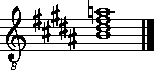
\includegraphics[height=1.15cm]{th-B7.cropped} & Bluesy. Lower 7th: A$\sharp$ $\to$ A. \\
\rowcolor{rowA}
\textbf{Bmaj7} & B major 7th & 1 -- 3 -- 5 -- 7 & 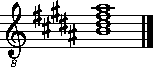
\includegraphics[height=1.15cm]{th-Bmaj7.cropped} & Dreamy, jazzy. Keep natural 7th (A$\sharp$). \\
\rowcolor{rowB}
\textbf{Bm7} & B minor 7th & 1 -- $\flat$3 -- 5 -- $\flat$7 & 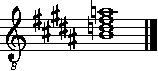
\includegraphics[height=1.15cm]{th-Bm7.cropped} & Mellow, soulful. Lower 3rd and 7th. \\
\rowcolor{rowA}
\textbf{Baug} & B augmented & 1 -- 3 -- $\sharp$5 & 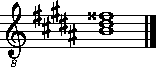
\includegraphics[height=1.15cm]{th-Baug.cropped} & Eerie. Raise the 5th by 1 semitone. \\
\rowcolor{rowB}
\textbf{Bdim} & B diminished & 1 -- $\flat$3 -- $\flat$5 & 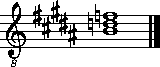
\includegraphics[height=1.15cm]{th-Bdim.cropped} & Very tense. Lower 3rd and 5th. \\
\rowcolor{rowA}
\textbf{Bdim7} & B dim. 7th & 1 -- $\flat$3 -- $\flat$5 -- $\flat\flat$7 & 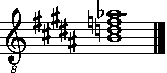
\includegraphics[height=1.15cm]{th-Bdim7.cropped} & Max. tense. All minor 3rds. \\
\rowcolor{rowB}
\textbf{Bm7$\flat$5} & B half-dim. & 1 -- $\flat$3 -- $\flat$5 -- $\flat$7 & 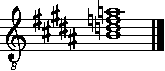
\includegraphics[height=1.15cm]{th-Bm7b5.cropped} & Tense, jazzy (also: B\o). \\
\bottomrule
\end{longtable}

\subsection*{The C Family}
\noindent\textbf{Key signature:} no sharps or flats.\smallskip

\begin{center}
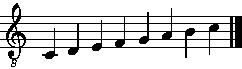
\includegraphics[height=1.15cm]{scale-C.cropped}\\[2pt]
{\small\color{mygray}\textbf{1} C\quad \textbf{2} D\quad \textbf{3} E\quad \textbf{4} F\quad \textbf{5} G\quad \textbf{6} A\quad \textbf{7} B\quad \textbf{8} C}
\end{center}

\begin{longtable}{@{}l l l c >{\raggedright\arraybackslash}p{4.4cm}@{}}
\toprule
\textbf{Symbol} & \textbf{Full name} & \textbf{Formula} & \textbf{Staff} & \textbf{Colour / use} \\
\midrule\endhead
\rowcolor{rowA}
\textbf{C} & C major & 1 -- 3 -- 5 & 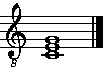
\includegraphics[height=1.15cm]{th-Cmaj.cropped} & Bright, stable. \\
\rowcolor{rowB}
\textbf{Cm} & C minor & 1 -- $\flat$3 -- 5 & 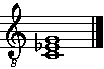
\includegraphics[height=1.15cm]{th-Cm.cropped} & Dark. Lower the 3rd: E $\to$ E$\flat$. \\
\rowcolor{rowA}
\textbf{C5} & C power chord & 1 -- 5 & 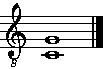
\includegraphics[height=1.15cm]{th-C5.cropped} & Raw, neutral. No 3rd. \\
\rowcolor{rowB}
\textbf{Csus2} & C sus. 2nd & 1 -- 2 -- 5 & 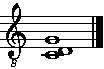
\includegraphics[height=1.15cm]{th-Csus2.cropped} & Open. Replace 3rd with 2nd (D). \\
\rowcolor{rowA}
\textbf{Csus4} & C sus. 4th & 1 -- 4 -- 5 & 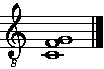
\includegraphics[height=1.15cm]{th-Csus4.cropped} & Tense. Replace 3rd with 4th (F). \\
\rowcolor{rowB}
\textbf{C6} & C major sixth & 1 -- 3 -- 5 -- 6 & 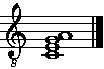
\includegraphics[height=1.15cm]{th-C6.cropped} & Sweet, vintage. Add 6th (A). \\
\rowcolor{rowA}
\textbf{Cadd9} & C add nine & 1 -- 3 -- 5 -- 9 & 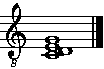
\includegraphics[height=1.15cm]{th-Cadd9.cropped} & Colourful. Add 2nd/9th (D), no 7th. \\
\rowcolor{rowB}
\textbf{C7} & C dominant 7th & 1 -- 3 -- 5 -- $\flat$7 & 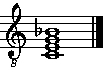
\includegraphics[height=1.15cm]{th-C7.cropped} & Bluesy. Lower 7th: B $\to$ B$\flat$. \\
\rowcolor{rowA}
\textbf{Cmaj7} & C major 7th & 1 -- 3 -- 5 -- 7 & 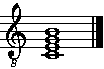
\includegraphics[height=1.15cm]{th-Cmaj7.cropped} & Dreamy, jazzy. Keep natural 7th (B). \\
\rowcolor{rowB}
\textbf{Cm7} & C minor 7th & 1 -- $\flat$3 -- 5 -- $\flat$7 & 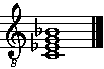
\includegraphics[height=1.15cm]{th-Cm7.cropped} & Mellow, soulful. Lower 3rd and 7th. \\
\rowcolor{rowA}
\textbf{Caug} & C augmented & 1 -- 3 -- $\sharp$5 & 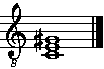
\includegraphics[height=1.15cm]{th-Caug.cropped} & Eerie. Raise the 5th by 1 semitone. \\
\rowcolor{rowB}
\textbf{Cdim} & C diminished & 1 -- $\flat$3 -- $\flat$5 & 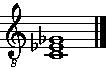
\includegraphics[height=1.15cm]{th-Cdim.cropped} & Very tense. Lower 3rd and 5th. \\
\rowcolor{rowA}
\textbf{Cdim7} & C dim. 7th & 1 -- $\flat$3 -- $\flat$5 -- $\flat\flat$7 & 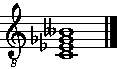
\includegraphics[height=1.15cm]{th-Cdim7.cropped} & Max. tense. All minor 3rds. \\
\rowcolor{rowB}
\textbf{Cm7$\flat$5} & C half-dim. & 1 -- $\flat$3 -- $\flat$5 -- $\flat$7 & 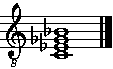
\includegraphics[height=1.15cm]{th-Cm7b5.cropped} & Tense, jazzy (also: C\o). \\
\bottomrule
\end{longtable}

\subsection*{The D Family}
\noindent\textbf{Key signature:} two sharps: F$\sharp$, C$\sharp$.\smallskip

\begin{center}
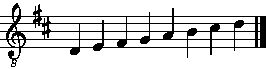
\includegraphics[height=1.15cm]{scale-D.cropped}\\[2pt]
{\small\color{mygray}\textbf{1} D\quad \textbf{2} E\quad \textbf{3} F$\sharp$\quad \textbf{4} G\quad \textbf{5} A\quad \textbf{6} B\quad \textbf{7} C$\sharp$\quad \textbf{8} D}
\end{center}

\begin{longtable}{@{}l l l c >{\raggedright\arraybackslash}p{4.4cm}@{}}
\toprule
\textbf{Symbol} & \textbf{Full name} & \textbf{Formula} & \textbf{Staff} & \textbf{Colour / use} \\
\midrule\endhead
\rowcolor{rowA}
\textbf{D} & D major & 1 -- 3 -- 5 & 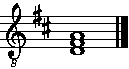
\includegraphics[height=1.15cm]{th-Dmaj.cropped} & Bright, stable. \\
\rowcolor{rowB}
\textbf{Dm} & D minor & 1 -- $\flat$3 -- 5 & 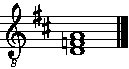
\includegraphics[height=1.15cm]{th-Dm.cropped} & Dark. Lower the 3rd: F$\sharp$ $\to$ F. \\
\rowcolor{rowA}
\textbf{D5} & D power chord & 1 -- 5 & 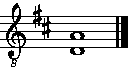
\includegraphics[height=1.15cm]{th-D5.cropped} & Raw, neutral. No 3rd. \\
\rowcolor{rowB}
\textbf{Dsus2} & D sus. 2nd & 1 -- 2 -- 5 & 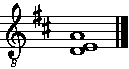
\includegraphics[height=1.15cm]{th-Dsus2.cropped} & Open. Replace 3rd with 2nd (E). \\
\rowcolor{rowA}
\textbf{Dsus4} & D sus. 4th & 1 -- 4 -- 5 & 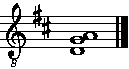
\includegraphics[height=1.15cm]{th-Dsus4.cropped} & Tense. Replace 3rd with 4th (G). \\
\rowcolor{rowB}
\textbf{D6} & D major sixth & 1 -- 3 -- 5 -- 6 & 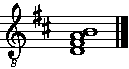
\includegraphics[height=1.15cm]{th-D6.cropped} & Sweet, vintage. Add 6th (B). \\
\rowcolor{rowA}
\textbf{Dadd9} & D add nine & 1 -- 3 -- 5 -- 9 & 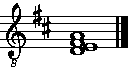
\includegraphics[height=1.15cm]{th-Dadd9.cropped} & Colourful. Add 2nd/9th (E), no 7th. \\
\rowcolor{rowB}
\textbf{D7} & D dominant 7th & 1 -- 3 -- 5 -- $\flat$7 & 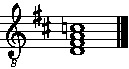
\includegraphics[height=1.15cm]{th-D7.cropped} & Bluesy. Lower 7th: C$\sharp$ $\to$ C. \\
\rowcolor{rowA}
\textbf{Dmaj7} & D major 7th & 1 -- 3 -- 5 -- 7 & 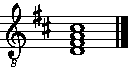
\includegraphics[height=1.15cm]{th-Dmaj7.cropped} & Dreamy, jazzy. Keep natural 7th (C$\sharp$). \\
\rowcolor{rowB}
\textbf{Dm7} & D minor 7th & 1 -- $\flat$3 -- 5 -- $\flat$7 & 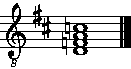
\includegraphics[height=1.15cm]{th-Dm7.cropped} & Mellow, soulful. Lower 3rd and 7th. \\
\rowcolor{rowA}
\textbf{Daug} & D augmented & 1 -- 3 -- $\sharp$5 & 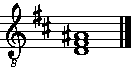
\includegraphics[height=1.15cm]{th-Daug.cropped} & Eerie. Raise the 5th by 1 semitone. \\
\rowcolor{rowB}
\textbf{Ddim} & D diminished & 1 -- $\flat$3 -- $\flat$5 & 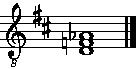
\includegraphics[height=1.15cm]{th-Ddim.cropped} & Very tense. Lower 3rd and 5th. \\
\rowcolor{rowA}
\textbf{Ddim7} & D dim. 7th & 1 -- $\flat$3 -- $\flat$5 -- $\flat\flat$7 & 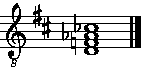
\includegraphics[height=1.15cm]{th-Ddim7.cropped} & Max. tense. All minor 3rds. \\
\rowcolor{rowB}
\textbf{Dm7$\flat$5} & D half-dim. & 1 -- $\flat$3 -- $\flat$5 -- $\flat$7 & 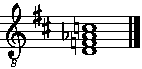
\includegraphics[height=1.15cm]{th-Dm7b5.cropped} & Tense, jazzy (also: D\o). \\
\bottomrule
\end{longtable}

\subsection*{The E Family}
\noindent\textbf{Key signature:} four sharps: F$\sharp$, C$\sharp$, G$\sharp$, D$\sharp$.\smallskip

\begin{center}
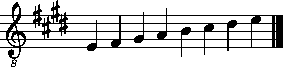
\includegraphics[height=1.15cm]{scale-E.cropped}\\[2pt]
{\small\color{mygray}\textbf{1} E\quad \textbf{2} F$\sharp$\quad \textbf{3} G$\sharp$\quad \textbf{4} A\quad \textbf{5} B\quad \textbf{6} C$\sharp$\quad \textbf{7} D$\sharp$\quad \textbf{8} E}
\end{center}

\begin{longtable}{@{}l l l c >{\raggedright\arraybackslash}p{4.4cm}@{}}
\toprule
\textbf{Symbol} & \textbf{Full name} & \textbf{Formula} & \textbf{Staff} & \textbf{Colour / use} \\
\midrule\endhead
\rowcolor{rowA}
\textbf{E} & E major & 1 -- 3 -- 5 & 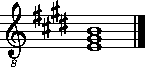
\includegraphics[height=1.15cm]{th-Emaj.cropped} & Bright, stable. \\
\rowcolor{rowB}
\textbf{Em} & E minor & 1 -- $\flat$3 -- 5 & 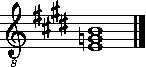
\includegraphics[height=1.15cm]{th-Em.cropped} & Dark. Lower the 3rd: G$\sharp$ $\to$ G. \\
\rowcolor{rowA}
\textbf{E5} & E power chord & 1 -- 5 & 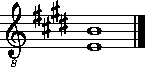
\includegraphics[height=1.15cm]{th-E5.cropped} & Raw, neutral. No 3rd. \\
\rowcolor{rowB}
\textbf{Esus2} & E sus. 2nd & 1 -- 2 -- 5 & 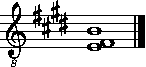
\includegraphics[height=1.15cm]{th-Esus2.cropped} & Open. Replace 3rd with 2nd (F$\sharp$). \\
\rowcolor{rowA}
\textbf{Esus4} & E sus. 4th & 1 -- 4 -- 5 & 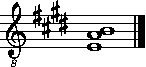
\includegraphics[height=1.15cm]{th-Esus4.cropped} & Tense. Replace 3rd with 4th (A). \\
\rowcolor{rowB}
\textbf{E6} & E major sixth & 1 -- 3 -- 5 -- 6 & 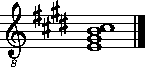
\includegraphics[height=1.15cm]{th-E6.cropped} & Sweet, vintage. Add 6th (C$\sharp$). \\
\rowcolor{rowA}
\textbf{Eadd9} & E add nine & 1 -- 3 -- 5 -- 9 & 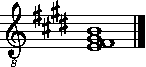
\includegraphics[height=1.15cm]{th-Eadd9.cropped} & Colourful. Add 2nd/9th (F$\sharp$), no 7th. \\
\rowcolor{rowB}
\textbf{E7} & E dominant 7th & 1 -- 3 -- 5 -- $\flat$7 & 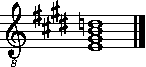
\includegraphics[height=1.15cm]{th-E7.cropped} & Bluesy. Lower 7th: D$\sharp$ $\to$ D. \\
\rowcolor{rowA}
\textbf{Emaj7} & E major 7th & 1 -- 3 -- 5 -- 7 & 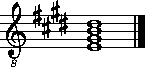
\includegraphics[height=1.15cm]{th-Emaj7.cropped} & Dreamy, jazzy. Keep natural 7th (D$\sharp$). \\
\rowcolor{rowB}
\textbf{Em7} & E minor 7th & 1 -- $\flat$3 -- 5 -- $\flat$7 & 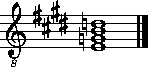
\includegraphics[height=1.15cm]{th-Em7.cropped} & Mellow, soulful. Lower 3rd and 7th. \\
\rowcolor{rowA}
\textbf{Eaug} & E augmented & 1 -- 3 -- $\sharp$5 & 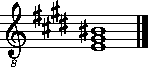
\includegraphics[height=1.15cm]{th-Eaug.cropped} & Eerie. Raise the 5th by 1 semitone. \\
\rowcolor{rowB}
\textbf{Edim} & E diminished & 1 -- $\flat$3 -- $\flat$5 & 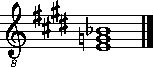
\includegraphics[height=1.15cm]{th-Edim.cropped} & Very tense. Lower 3rd and 5th. \\
\rowcolor{rowA}
\textbf{Edim7} & E dim. 7th & 1 -- $\flat$3 -- $\flat$5 -- $\flat\flat$7 & 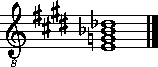
\includegraphics[height=1.15cm]{th-Edim7.cropped} & Max. tense. All minor 3rds. \\
\rowcolor{rowB}
\textbf{Em7$\flat$5} & E half-dim. & 1 -- $\flat$3 -- $\flat$5 -- $\flat$7 & 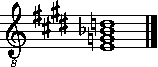
\includegraphics[height=1.15cm]{th-Em7b5.cropped} & Tense, jazzy (also: E\o). \\
\bottomrule
\end{longtable}

\subsection*{The F Family}
\noindent\textbf{Key signature:} one flat: B$\flat$.\smallskip

\begin{center}
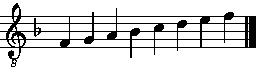
\includegraphics[height=1.15cm]{scale-F.cropped}\\[2pt]
{\small\color{mygray}\textbf{1} F\quad \textbf{2} G\quad \textbf{3} A\quad \textbf{4} B$\flat$\quad \textbf{5} C\quad \textbf{6} D\quad \textbf{7} E\quad \textbf{8} F}
\end{center}

\begin{longtable}{@{}l l l c >{\raggedright\arraybackslash}p{4.4cm}@{}}
\toprule
\textbf{Symbol} & \textbf{Full name} & \textbf{Formula} & \textbf{Staff} & \textbf{Colour / use} \\
\midrule\endhead
\rowcolor{rowA}
\textbf{F} & F major & 1 -- 3 -- 5 & 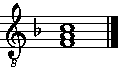
\includegraphics[height=1.15cm]{th-Fmaj.cropped} & Bright, stable. \\
\rowcolor{rowB}
\textbf{Fm} & F minor & 1 -- $\flat$3 -- 5 & 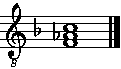
\includegraphics[height=1.15cm]{th-Fm.cropped} & Dark. Lower the 3rd: A $\to$ A$\flat$. \\
\rowcolor{rowA}
\textbf{F5} & F power chord & 1 -- 5 & 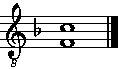
\includegraphics[height=1.15cm]{th-F5.cropped} & Raw, neutral. No 3rd. \\
\rowcolor{rowB}
\textbf{Fsus2} & F sus. 2nd & 1 -- 2 -- 5 & 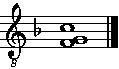
\includegraphics[height=1.15cm]{th-Fsus2.cropped} & Open. Replace 3rd with 2nd (G). \\
\rowcolor{rowA}
\textbf{Fsus4} & F sus. 4th & 1 -- 4 -- 5 & 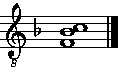
\includegraphics[height=1.15cm]{th-Fsus4.cropped} & Tense. Replace 3rd with 4th (B$\flat$). \\
\rowcolor{rowB}
\textbf{F6} & F major sixth & 1 -- 3 -- 5 -- 6 & 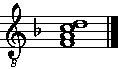
\includegraphics[height=1.15cm]{th-F6.cropped} & Sweet, vintage. Add 6th (D). \\
\rowcolor{rowA}
\textbf{Fadd9} & F add nine & 1 -- 3 -- 5 -- 9 & 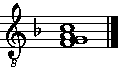
\includegraphics[height=1.15cm]{th-Fadd9.cropped} & Colourful. Add 2nd/9th (G), no 7th. \\
\rowcolor{rowB}
\textbf{F7} & F dominant 7th & 1 -- 3 -- 5 -- $\flat$7 & 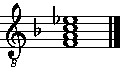
\includegraphics[height=1.15cm]{th-F7.cropped} & Bluesy. Lower 7th: E $\to$ E$\flat$. \\
\rowcolor{rowA}
\textbf{Fmaj7} & F major 7th & 1 -- 3 -- 5 -- 7 & 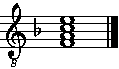
\includegraphics[height=1.15cm]{th-Fmaj7.cropped} & Dreamy, jazzy. Keep natural 7th (E). \\
\rowcolor{rowB}
\textbf{Fm7} & F minor 7th & 1 -- $\flat$3 -- 5 -- $\flat$7 & 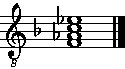
\includegraphics[height=1.15cm]{th-Fm7.cropped} & Mellow, soulful. Lower 3rd and 7th. \\
\rowcolor{rowA}
\textbf{Faug} & F augmented & 1 -- 3 -- $\sharp$5 & 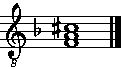
\includegraphics[height=1.15cm]{th-Faug.cropped} & Eerie. Raise the 5th by 1 semitone. \\
\rowcolor{rowB}
\textbf{Fdim} & F diminished & 1 -- $\flat$3 -- $\flat$5 & 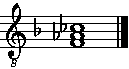
\includegraphics[height=1.15cm]{th-Fdim.cropped} & Very tense. Lower 3rd and 5th. \\
\rowcolor{rowA}
\textbf{Fdim7} & F dim. 7th & 1 -- $\flat$3 -- $\flat$5 -- $\flat\flat$7 & 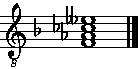
\includegraphics[height=1.15cm]{th-Fdim7.cropped} & Max. tense. All minor 3rds. \\
\rowcolor{rowB}
\textbf{Fm7$\flat$5} & F half-dim. & 1 -- $\flat$3 -- $\flat$5 -- $\flat$7 & 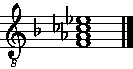
\includegraphics[height=1.15cm]{th-Fm7b5.cropped} & Tense, jazzy (also: F\o). \\
\bottomrule
\end{longtable}

\subsection*{The G Family}
\noindent\textbf{Key signature:} one sharp: F$\sharp$.\smallskip

\begin{center}
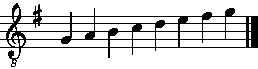
\includegraphics[height=1.15cm]{scale-G.cropped}\\[2pt]
{\small\color{mygray}\textbf{1} G\quad \textbf{2} A\quad \textbf{3} B\quad \textbf{4} C\quad \textbf{5} D\quad \textbf{6} E\quad \textbf{7} F$\sharp$\quad \textbf{8} G}
\end{center}

\begin{longtable}{@{}l l l c >{\raggedright\arraybackslash}p{4.4cm}@{}}
\toprule
\textbf{Symbol} & \textbf{Full name} & \textbf{Formula} & \textbf{Staff} & \textbf{Colour / use} \\
\midrule\endhead
\rowcolor{rowA}
\textbf{G} & G major & 1 -- 3 -- 5 & 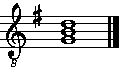
\includegraphics[height=1.15cm]{th-Gmaj.cropped} & Bright, stable. \\
\rowcolor{rowB}
\textbf{Gm} & G minor & 1 -- $\flat$3 -- 5 & 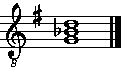
\includegraphics[height=1.15cm]{th-Gm.cropped} & Dark. Lower the 3rd: B $\to$ B$\flat$. \\
\rowcolor{rowA}
\textbf{G5} & G power chord & 1 -- 5 & 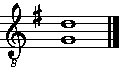
\includegraphics[height=1.15cm]{th-G5.cropped} & Raw, neutral. No 3rd. \\
\rowcolor{rowB}
\textbf{Gsus2} & G sus. 2nd & 1 -- 2 -- 5 & 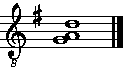
\includegraphics[height=1.15cm]{th-Gsus2.cropped} & Open. Replace 3rd with 2nd (A). \\
\rowcolor{rowA}
\textbf{Gsus4} & G sus. 4th & 1 -- 4 -- 5 & 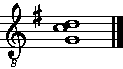
\includegraphics[height=1.15cm]{th-Gsus4.cropped} & Tense. Replace 3rd with 4th (C). \\
\rowcolor{rowB}
\textbf{G6} & G major sixth & 1 -- 3 -- 5 -- 6 & 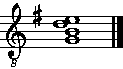
\includegraphics[height=1.15cm]{th-G6.cropped} & Sweet, vintage. Add 6th (E). \\
\rowcolor{rowA}
\textbf{Gadd9} & G add nine & 1 -- 3 -- 5 -- 9 & 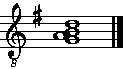
\includegraphics[height=1.15cm]{th-Gadd9.cropped} & Colourful. Add 2nd/9th (A), no 7th. \\
\rowcolor{rowB}
\textbf{G7} & G dominant 7th & 1 -- 3 -- 5 -- $\flat$7 & 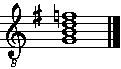
\includegraphics[height=1.15cm]{th-G7.cropped} & Bluesy. Lower 7th: F$\sharp$ $\to$ F. \\
\rowcolor{rowA}
\textbf{Gmaj7} & G major 7th & 1 -- 3 -- 5 -- 7 & 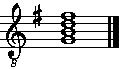
\includegraphics[height=1.15cm]{th-Gmaj7.cropped} & Dreamy, jazzy. Keep natural 7th (F$\sharp$). \\
\rowcolor{rowB}
\textbf{Gm7} & G minor 7th & 1 -- $\flat$3 -- 5 -- $\flat$7 & 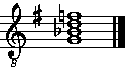
\includegraphics[height=1.15cm]{th-Gm7.cropped} & Mellow, soulful. Lower 3rd and 7th. \\
\rowcolor{rowA}
\textbf{Gaug} & G augmented & 1 -- 3 -- $\sharp$5 & 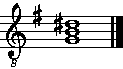
\includegraphics[height=1.15cm]{th-Gaug.cropped} & Eerie. Raise the 5th by 1 semitone. \\
\rowcolor{rowB}
\textbf{Gdim} & G diminished & 1 -- $\flat$3 -- $\flat$5 & 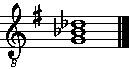
\includegraphics[height=1.15cm]{th-Gdim.cropped} & Very tense. Lower 3rd and 5th. \\
\rowcolor{rowA}
\textbf{Gdim7} & G dim. 7th & 1 -- $\flat$3 -- $\flat$5 -- $\flat\flat$7 & 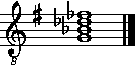
\includegraphics[height=1.15cm]{th-Gdim7.cropped} & Max. tense. All minor 3rds. \\
\rowcolor{rowB}
\textbf{Gm7$\flat$5} & G half-dim. & 1 -- $\flat$3 -- $\flat$5 -- $\flat$7 & 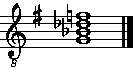
\includegraphics[height=1.15cm]{th-Gm7b5.cropped} & Tense, jazzy (also: G\o). \\
\bottomrule
\end{longtable}

